\section{Diagrama de Contexto}

\begin{figure}[h!]
  	\centering
	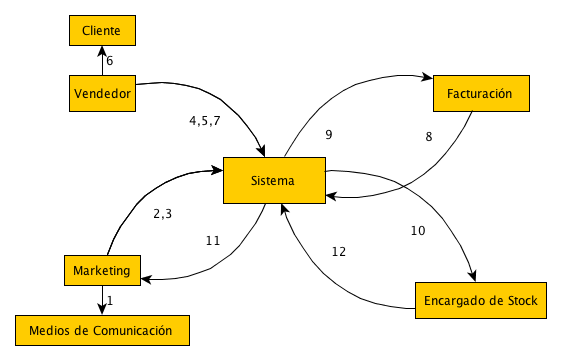
\includegraphics[width=0.8\textwidth]{./imagenes/diagrama_contexto.png}
	\caption{Diagrama de Contexto para Sistema de Venta de Celulares}
\end{figure}

\subsection{Referencias}

\begin{enumerate}

	\item Marketing monitorea promociones de la competencia para crear ofertas competitivas.
	 
	\item Marketing revisa el estado actual del stock en el sistema.
	 
	\item Marketing carga las promociones en el sistema.
	 
	\item Vendedor consulta información del cliente al sistema.
	 
	\item Vendedor consulta promociones disponibles en sistema.
	 
	\item Vendedor negocia con Cliente y finalmente vende (o no).
	 
	\item Vendedor registra la venta en el sistema.
	 
	\item Sistema notifica venta a Facturación para que sea procesada.
	 
	\item Facturación valida venta en sistema.
	 
	\item Sistema avisa a Encargado de Stock que debe despachar una venta.

	\item Sistema avisa a Marketing de los productos con stock excedente / nuevos celulares en mercado.

	\item Encargado de Stock registra en Sistema la mercadería que ingresa.

\end{enumerate}
